% !TeX program = xelatex
\documentclass[UTF8,a4paper,12pt]{ctexart}

\usepackage[margin=2.2cm]{geometry}
\usepackage{graphicx}
\usepackage{booktabs}
\usepackage{float}
\usepackage{subcaption}
\usepackage{amsmath}
\usepackage{amssymb}
\usepackage{xcolor}
\usepackage{listings}
\usepackage{hyperref}

\graphicspath{{./}{outputs/}{outputs/task1_histograms/}{outputs/task2_equalization/}{outputs/task3_hist_matching/}{outputs/task4_local_7x7/}{outputs/task5_segmentation/}}

\hypersetup{
  colorlinks=true,
  linkcolor=blue,
  urlcolor=blue,
  citecolor=blue
}

\lstdefinestyle{py}{
  language=Python,
  basicstyle=\ttfamily\small,
  keywordstyle=\color{blue!70!black},
  commentstyle=\color{green!40!black},
  stringstyle=\color{orange!60!black},
  numbers=left,
  numberstyle=\tiny\color{gray},
  stepnumber=1,
  numbersep=8pt,
  frame=single,
  breaklines=true,
  tabsize=4,
  showstringspaces=false
}

\title{视频图像处理实验报告\\第三次作业：直方图图像增强}
\author{姓名：\underline{\hspace{3cm}} \quad 学号：\underline{\hspace{3cm}}}
\date{\today}

\begin{document}
\maketitle
\tableofcontents
\newpage

\section{实验目的}
\begin{enumerate}
  \item 掌握图像直方图的统计意义及可视化方法。
  \item 实现全局直方图均衡与直方图匹配，并比较增强效果。
  \item 实现局部直方图增强（$7\times 7$）。
  \item 基于直方图阈值方法完成图像分割。
\end{enumerate}

\section{实验环境与数据}
\subsection{实验环境}
\begin{itemize}
  \item 操作系统：Windows
  \item 编程语言：Python 3
  \item 主要库：NumPy、Pillow、Matplotlib、scikit-image、pandas
\end{itemize}

\subsection{实验数据}
本次实验使用 14 幅 BMP 图像：\texttt{citywall*}、\texttt{elain*}、\texttt{lena*}、\texttt{woman*}（其中无数字后缀图像作为参考原图）。

\section{实验任务}
\begin{enumerate}
  \item 绘制所有附件图像直方图；
  \item 对所有图像做直方图均衡并输出对比；
  \item 自行指定目标直方图进行直方图匹配；
  \item 对 \texttt{elain} 和 \texttt{lena} 做 $7\times7$ 局部直方图增强；
  \item 利用直方图对 \texttt{elain} 和 \texttt{woman} 进行分割。
\end{enumerate}

\section{实验原理}
\subsection{直方图均衡}
设灰度图像灰度级为 $r_k$，其概率分布为 $p(r_k)$。均衡化通过变换
\begin{equation}
s_k = T(r_k)=\sum_{j=0}^{k}p(r_j)
\end{equation}
将原始灰度分布拉伸到更均匀的区间，从而提升整体对比度。

\subsection{直方图匹配}
给定源图像灰度映射 $T_s$ 和参考图像灰度映射 $T_r$，匹配目标是找到变换使源图像的累计分布逼近参考图像累计分布。

\subsection{局部直方图增强}
在每个像素邻域（本实验为 $7\times7$ 窗口）进行局部均衡，可提升局部对比度和细节纹理。

\subsection{基于直方图阈值分割}
\begin{itemize}
  \item Otsu：自动寻找使类间方差最大的单阈值；
  \item Multi-Otsu：扩展到多阈值分割，适合多峰分布图像。
\end{itemize}

\section{关键代码}
\subsection{全局直方图均衡}
\begin{lstlisting}[style=py]
def equalize_global(img_u8: np.ndarray) -> np.ndarray:
    out = exposure.equalize_hist(img_u8)
    return np.clip(np.round(out * 255.0), 0, 255).astype(np.uint8)
\end{lstlisting}

\subsection{直方图匹配}
\begin{lstlisting}[style=py]
matched = exposure.match_histograms(src, ref, channel_axis=None)
matched_u8 = np.clip(np.round(matched), 0, 255).astype(np.uint8)
\end{lstlisting}

\subsection{7x7 局部增强}
\begin{lstlisting}[style=py]
from skimage.filters.rank import equalize as rank_equalize
from skimage.morphology import footprint_rectangle

out = rank_equalize(img_u8, footprint=footprint_rectangle((7, 7)))
\end{lstlisting}

\subsection{分割阈值}
\begin{lstlisting}[style=py]
th = filters.threshold_otsu(elain_img)
ths = filters.threshold_multiotsu(woman_img, classes=3)
\end{lstlisting}

\section{实验结果与分析}
\subsection{任务1：直方图绘制}
\begin{figure}[H]
  \centering
  \begin{subfigure}{0.48\textwidth}
    \centering
    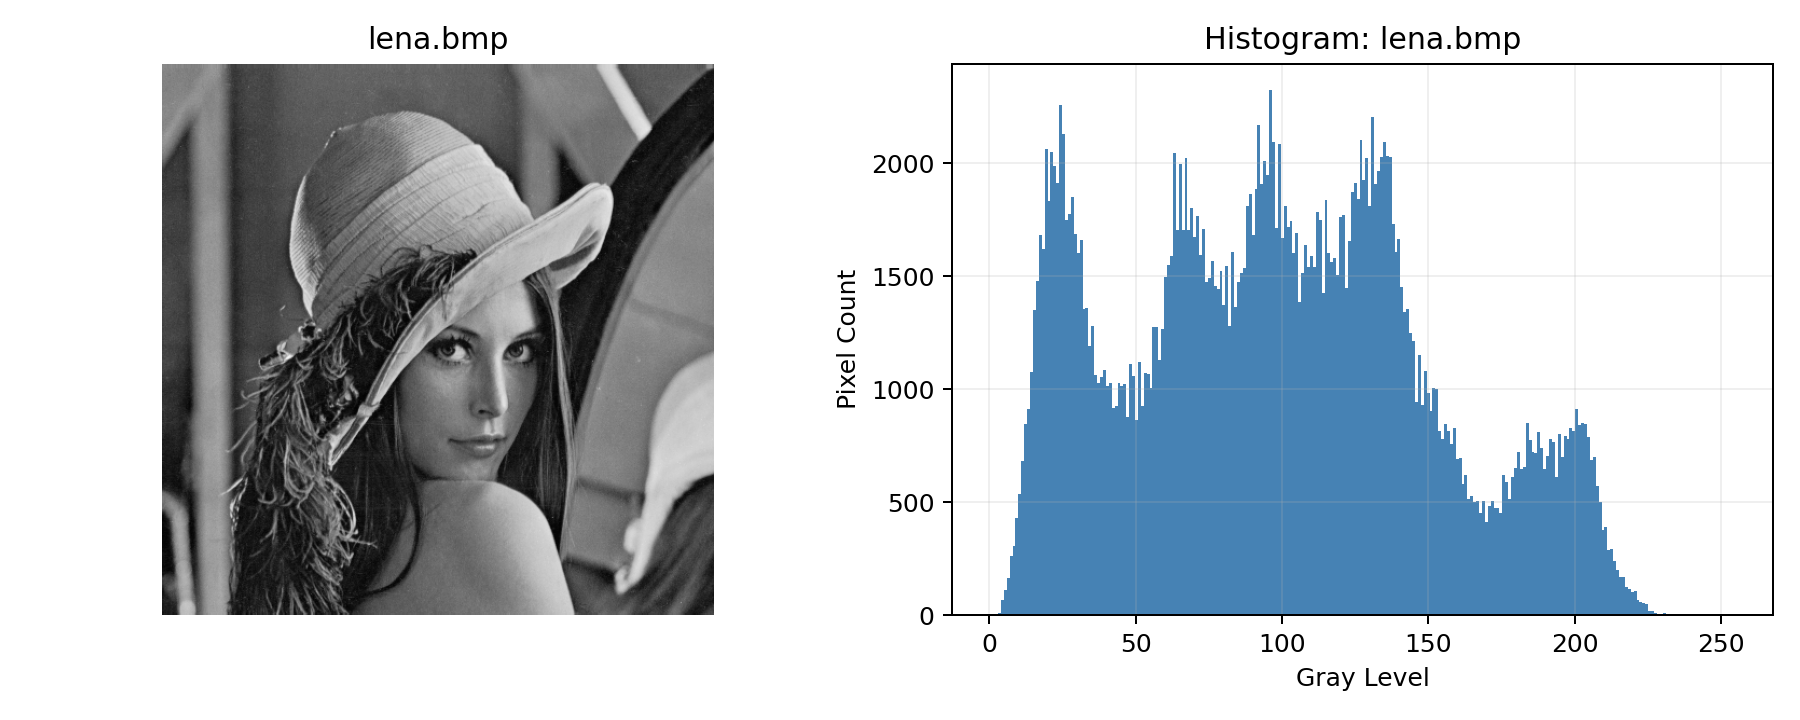
\includegraphics[width=\linewidth]{lena.bmp_img_hist.png}
    \caption{lena.bmp 图像与直方图}
  \end{subfigure}
  \begin{subfigure}{0.48\textwidth}
    \centering
    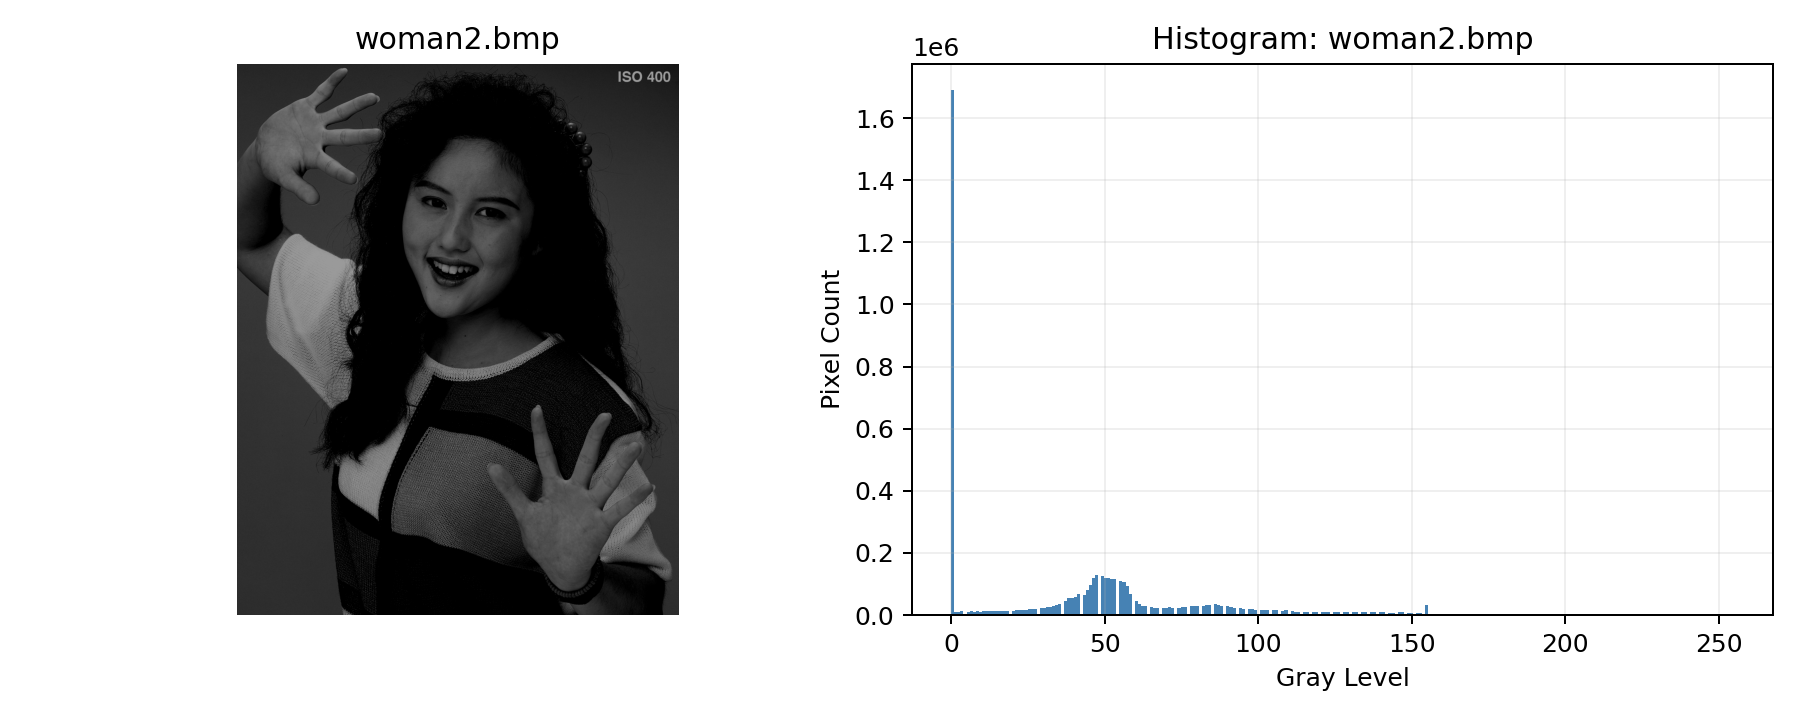
\includegraphics[width=\linewidth]{woman2.bmp_img_hist.png}
    \caption{woman2.bmp 图像与直方图}
  \end{subfigure}
  \caption{任务1结果示例（其余图像见 \texttt{outputs/task1\_histograms}）}
\end{figure}

\subsection{任务2：全局直方图均衡}
\begin{figure}[H]
  \centering
  \begin{subfigure}{0.49\textwidth}
    \centering
    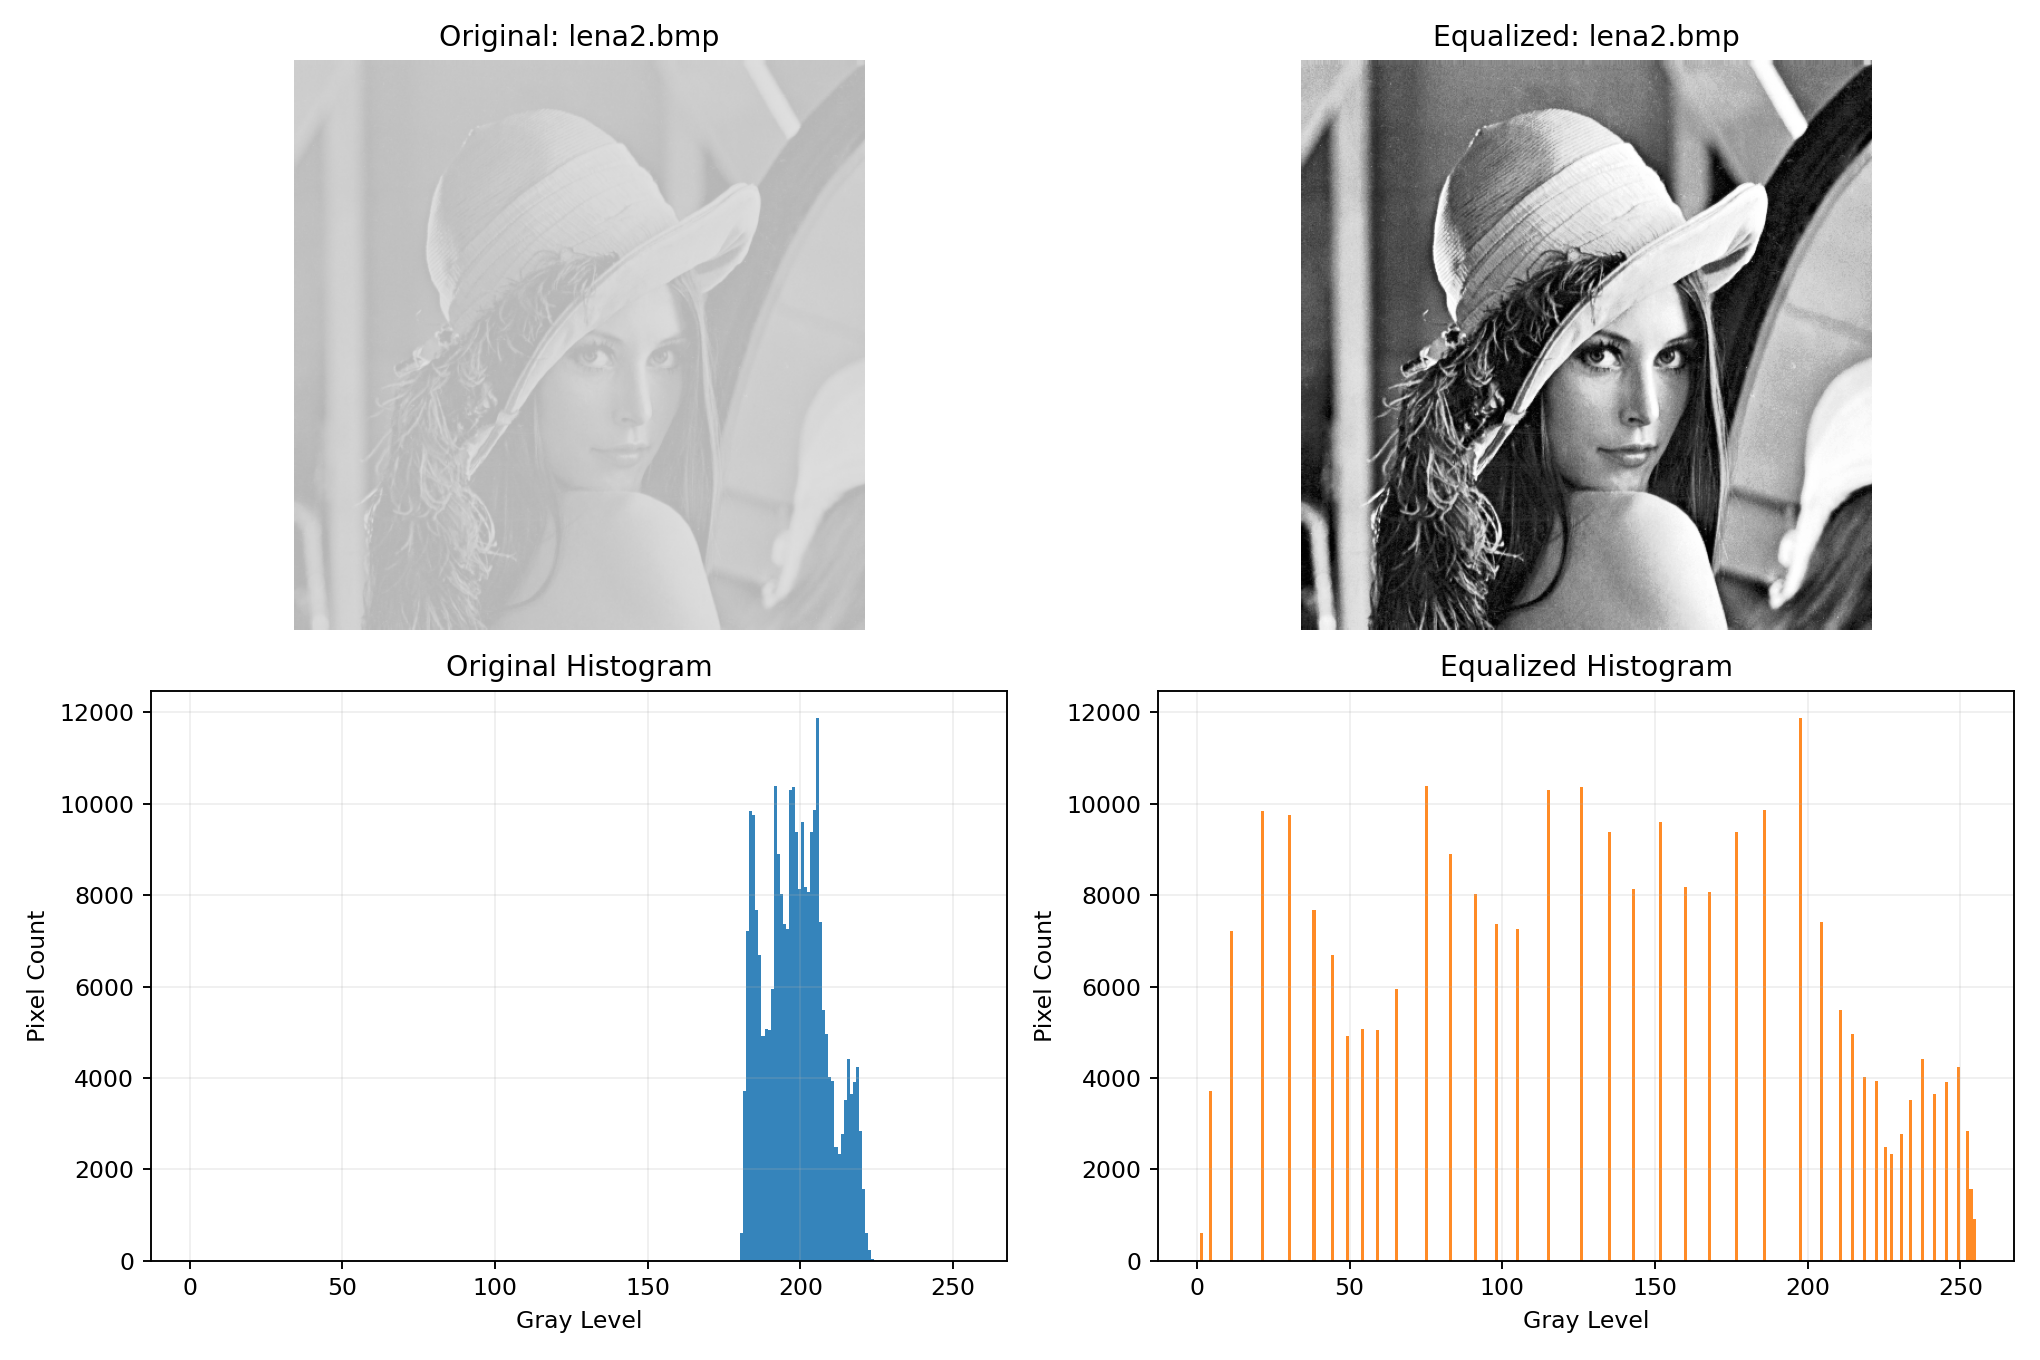
\includegraphics[width=\linewidth]{lena2.bmp_comparison.png}
    \caption{lena2.bmp}
  \end{subfigure}
  \begin{subfigure}{0.49\textwidth}
    \centering
    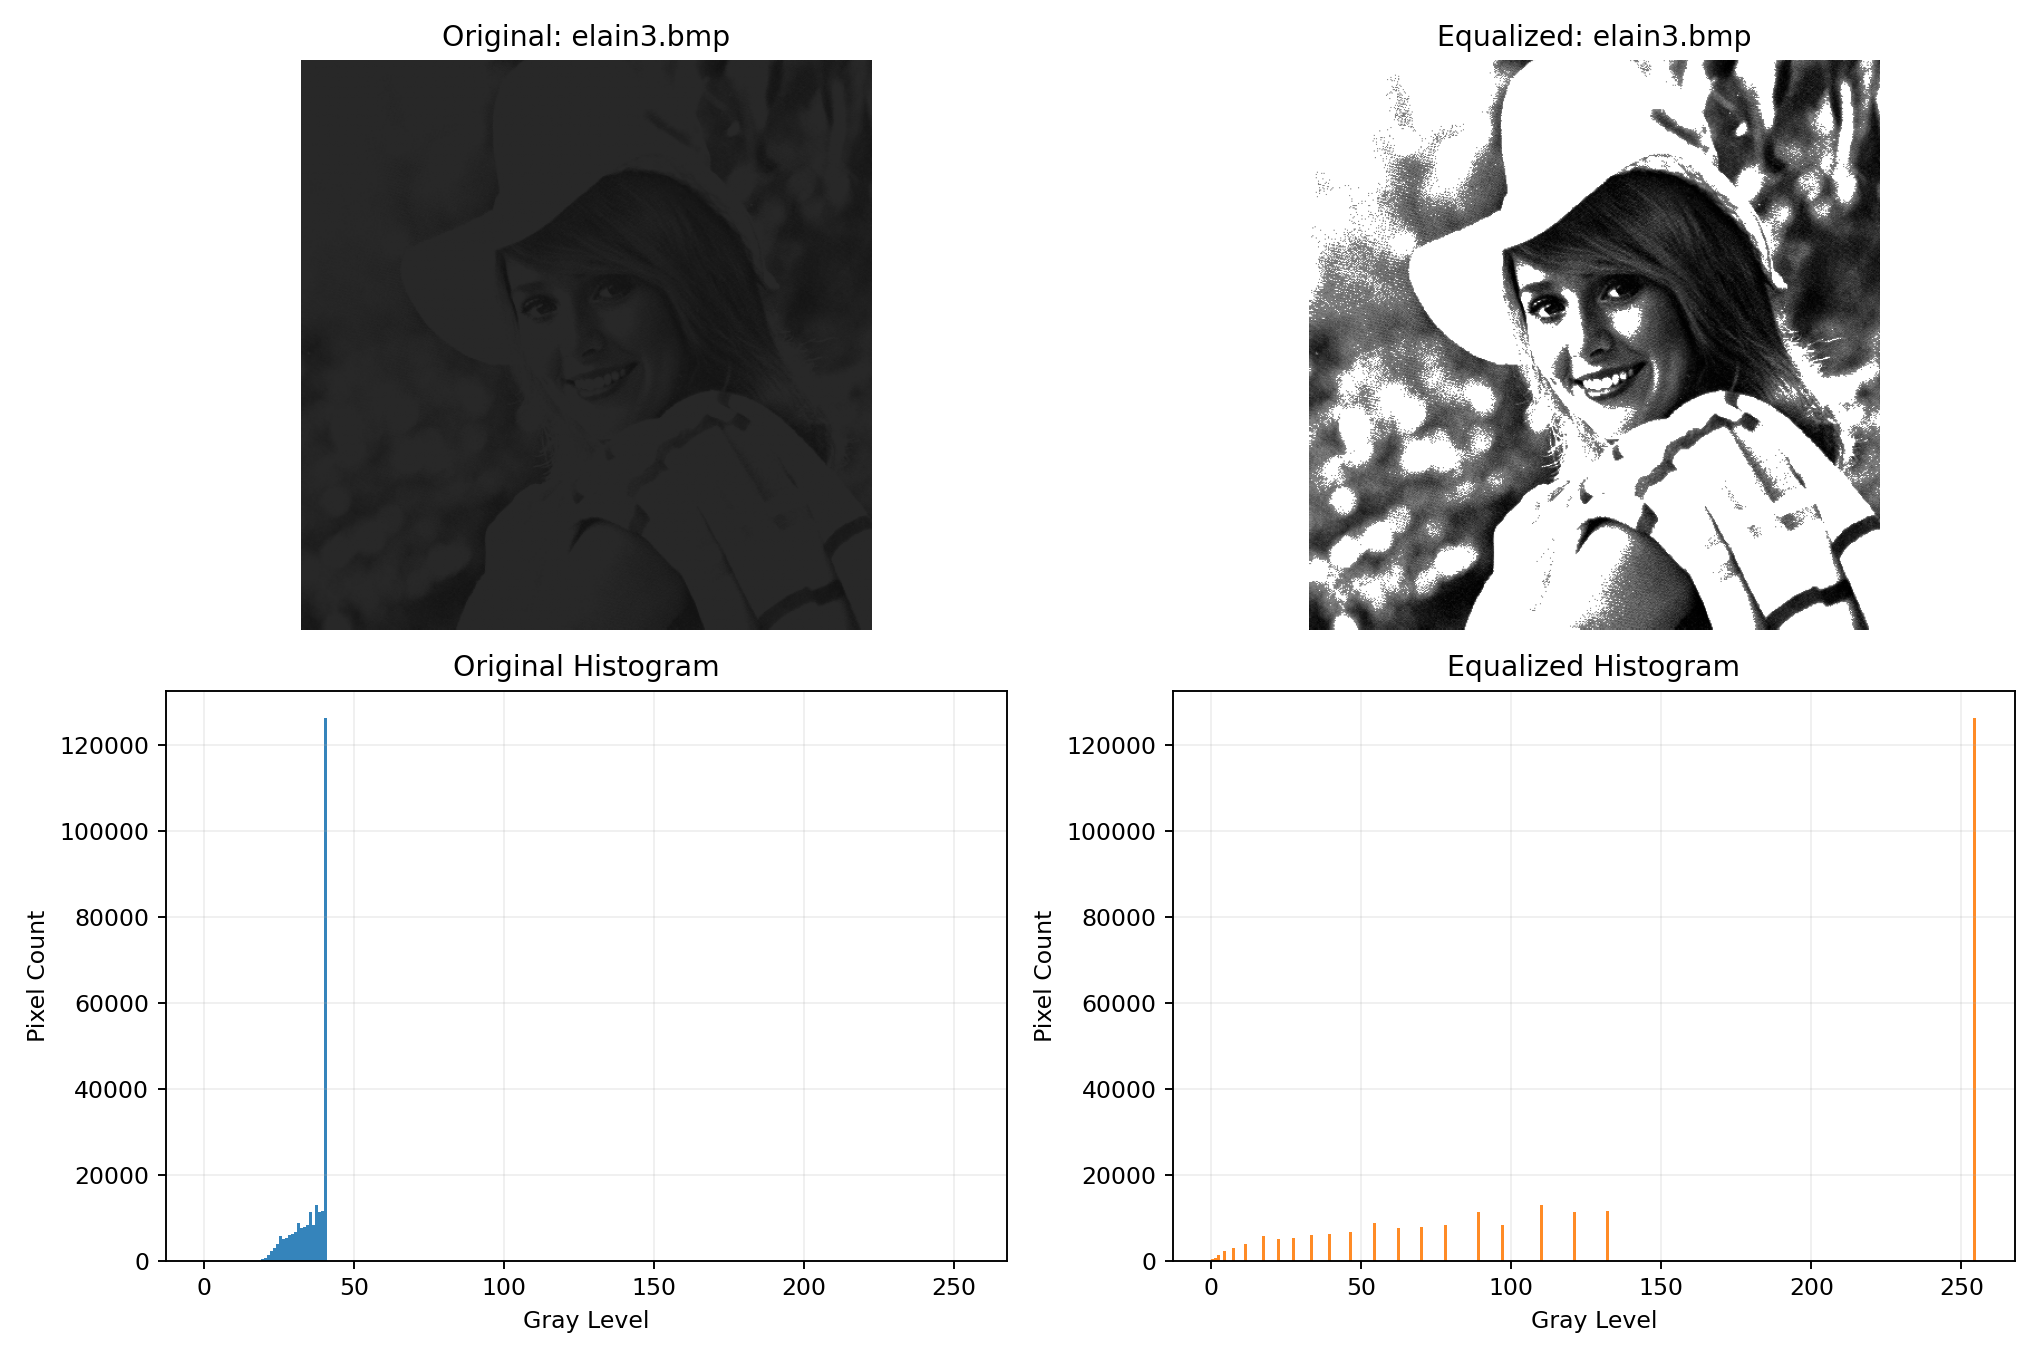
\includegraphics[width=\linewidth]{elain3.bmp_comparison.png}
    \caption{elain3.bmp}
  \end{subfigure}

  \vspace{0.5em}
  \begin{subfigure}{0.49\textwidth}
    \centering
    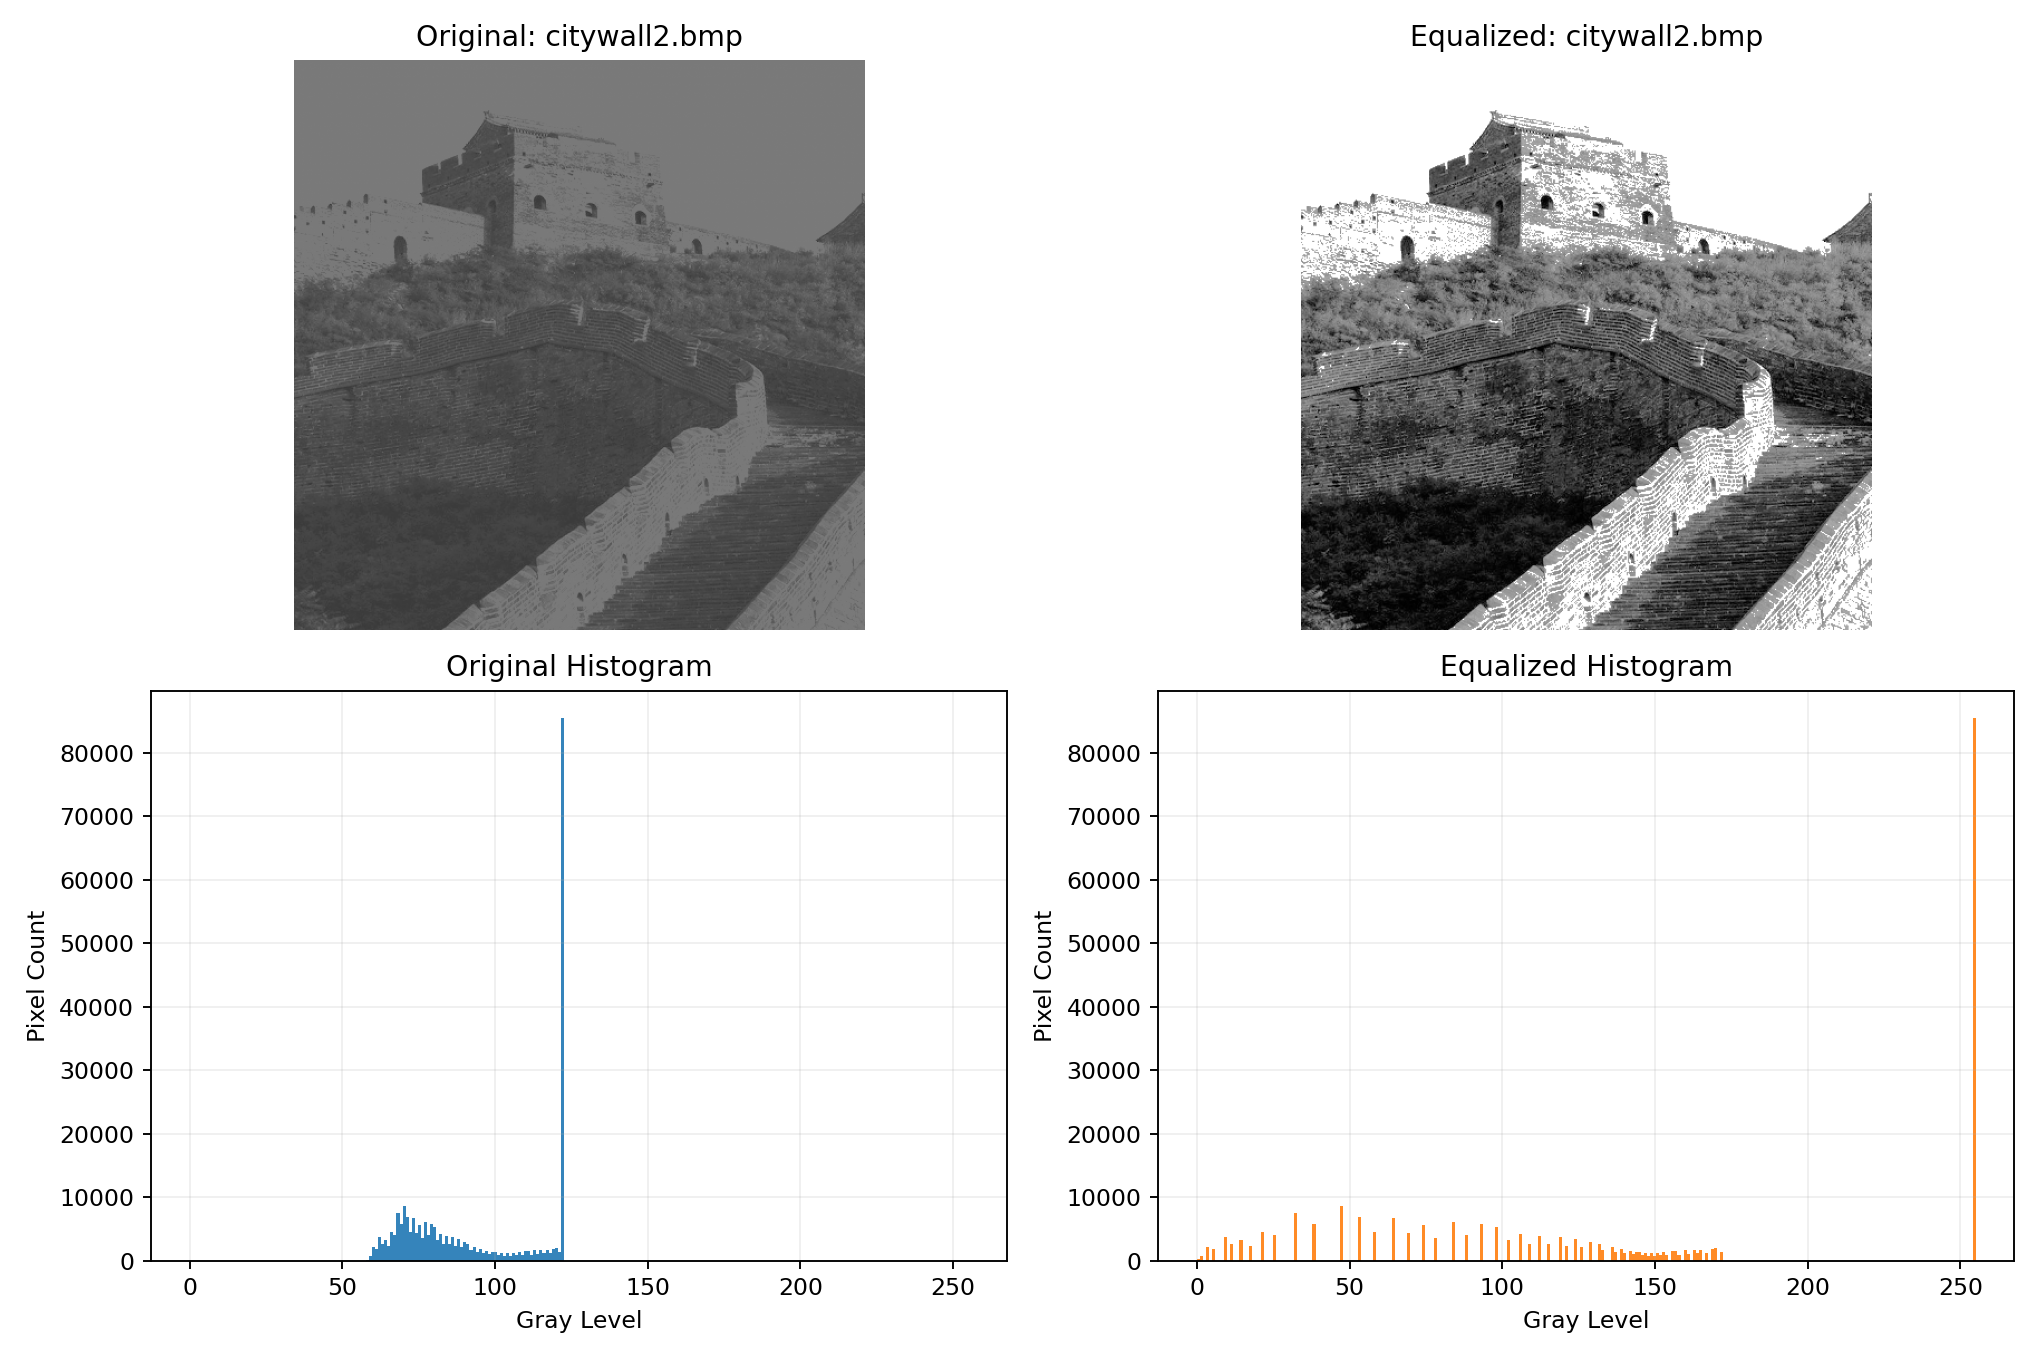
\includegraphics[width=\linewidth]{citywall2.bmp_comparison.png}
    \caption{citywall2.bmp}
  \end{subfigure}
  \begin{subfigure}{0.49\textwidth}
    \centering
    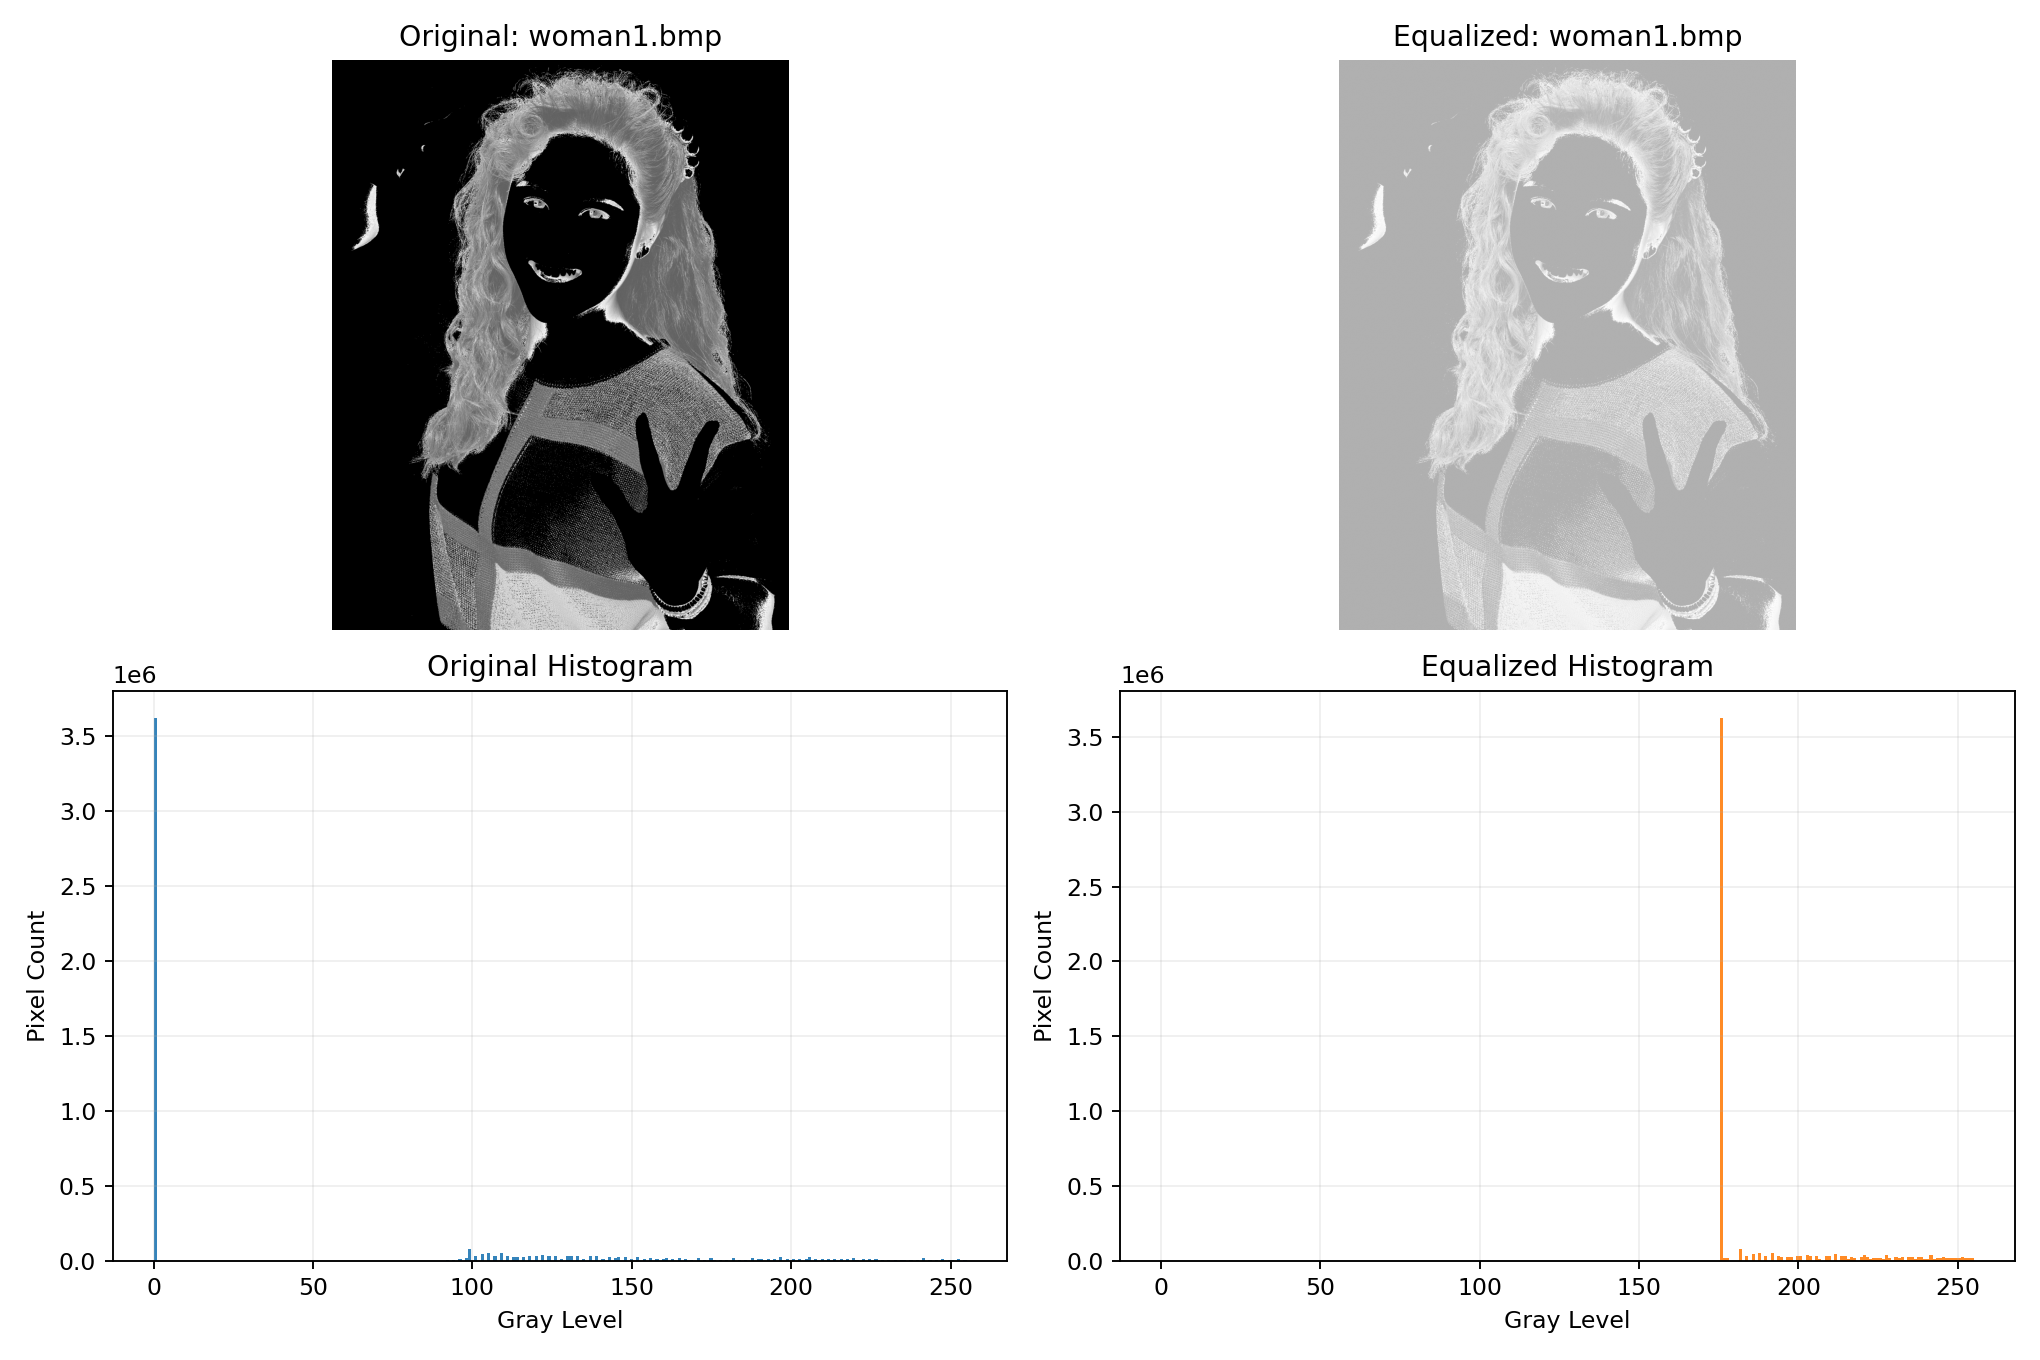
\includegraphics[width=\linewidth]{woman1.bmp_comparison.png}
    \caption{woman1.bmp}
  \end{subfigure}
  \caption{任务2：均衡化前后对比示例}
\end{figure}

\begin{table}[H]
\centering
\caption{任务2关键统计（部分）}
\begin{tabular}{lccc}
\toprule
图像 & 原始std & 均衡后std & 现象 \\
\midrule
citywall2.bmp & 22.781 & 88.083 & 对比度显著提升 \\
lena2.bmp & 10.159 & 73.235 & 灰度范围明显拉伸 \\
elain3.bmp & 5.292 & 96.627 & 低对比度得到强化 \\
woman1.bmp & 75.404 & 22.418 & 过暗/双峰图像被压缩 \\
\bottomrule
\end{tabular}
\end{table}

\subsection{任务3：直方图匹配}
\begin{figure}[H]
  \centering
  \begin{subfigure}{0.49\textwidth}
    \centering
    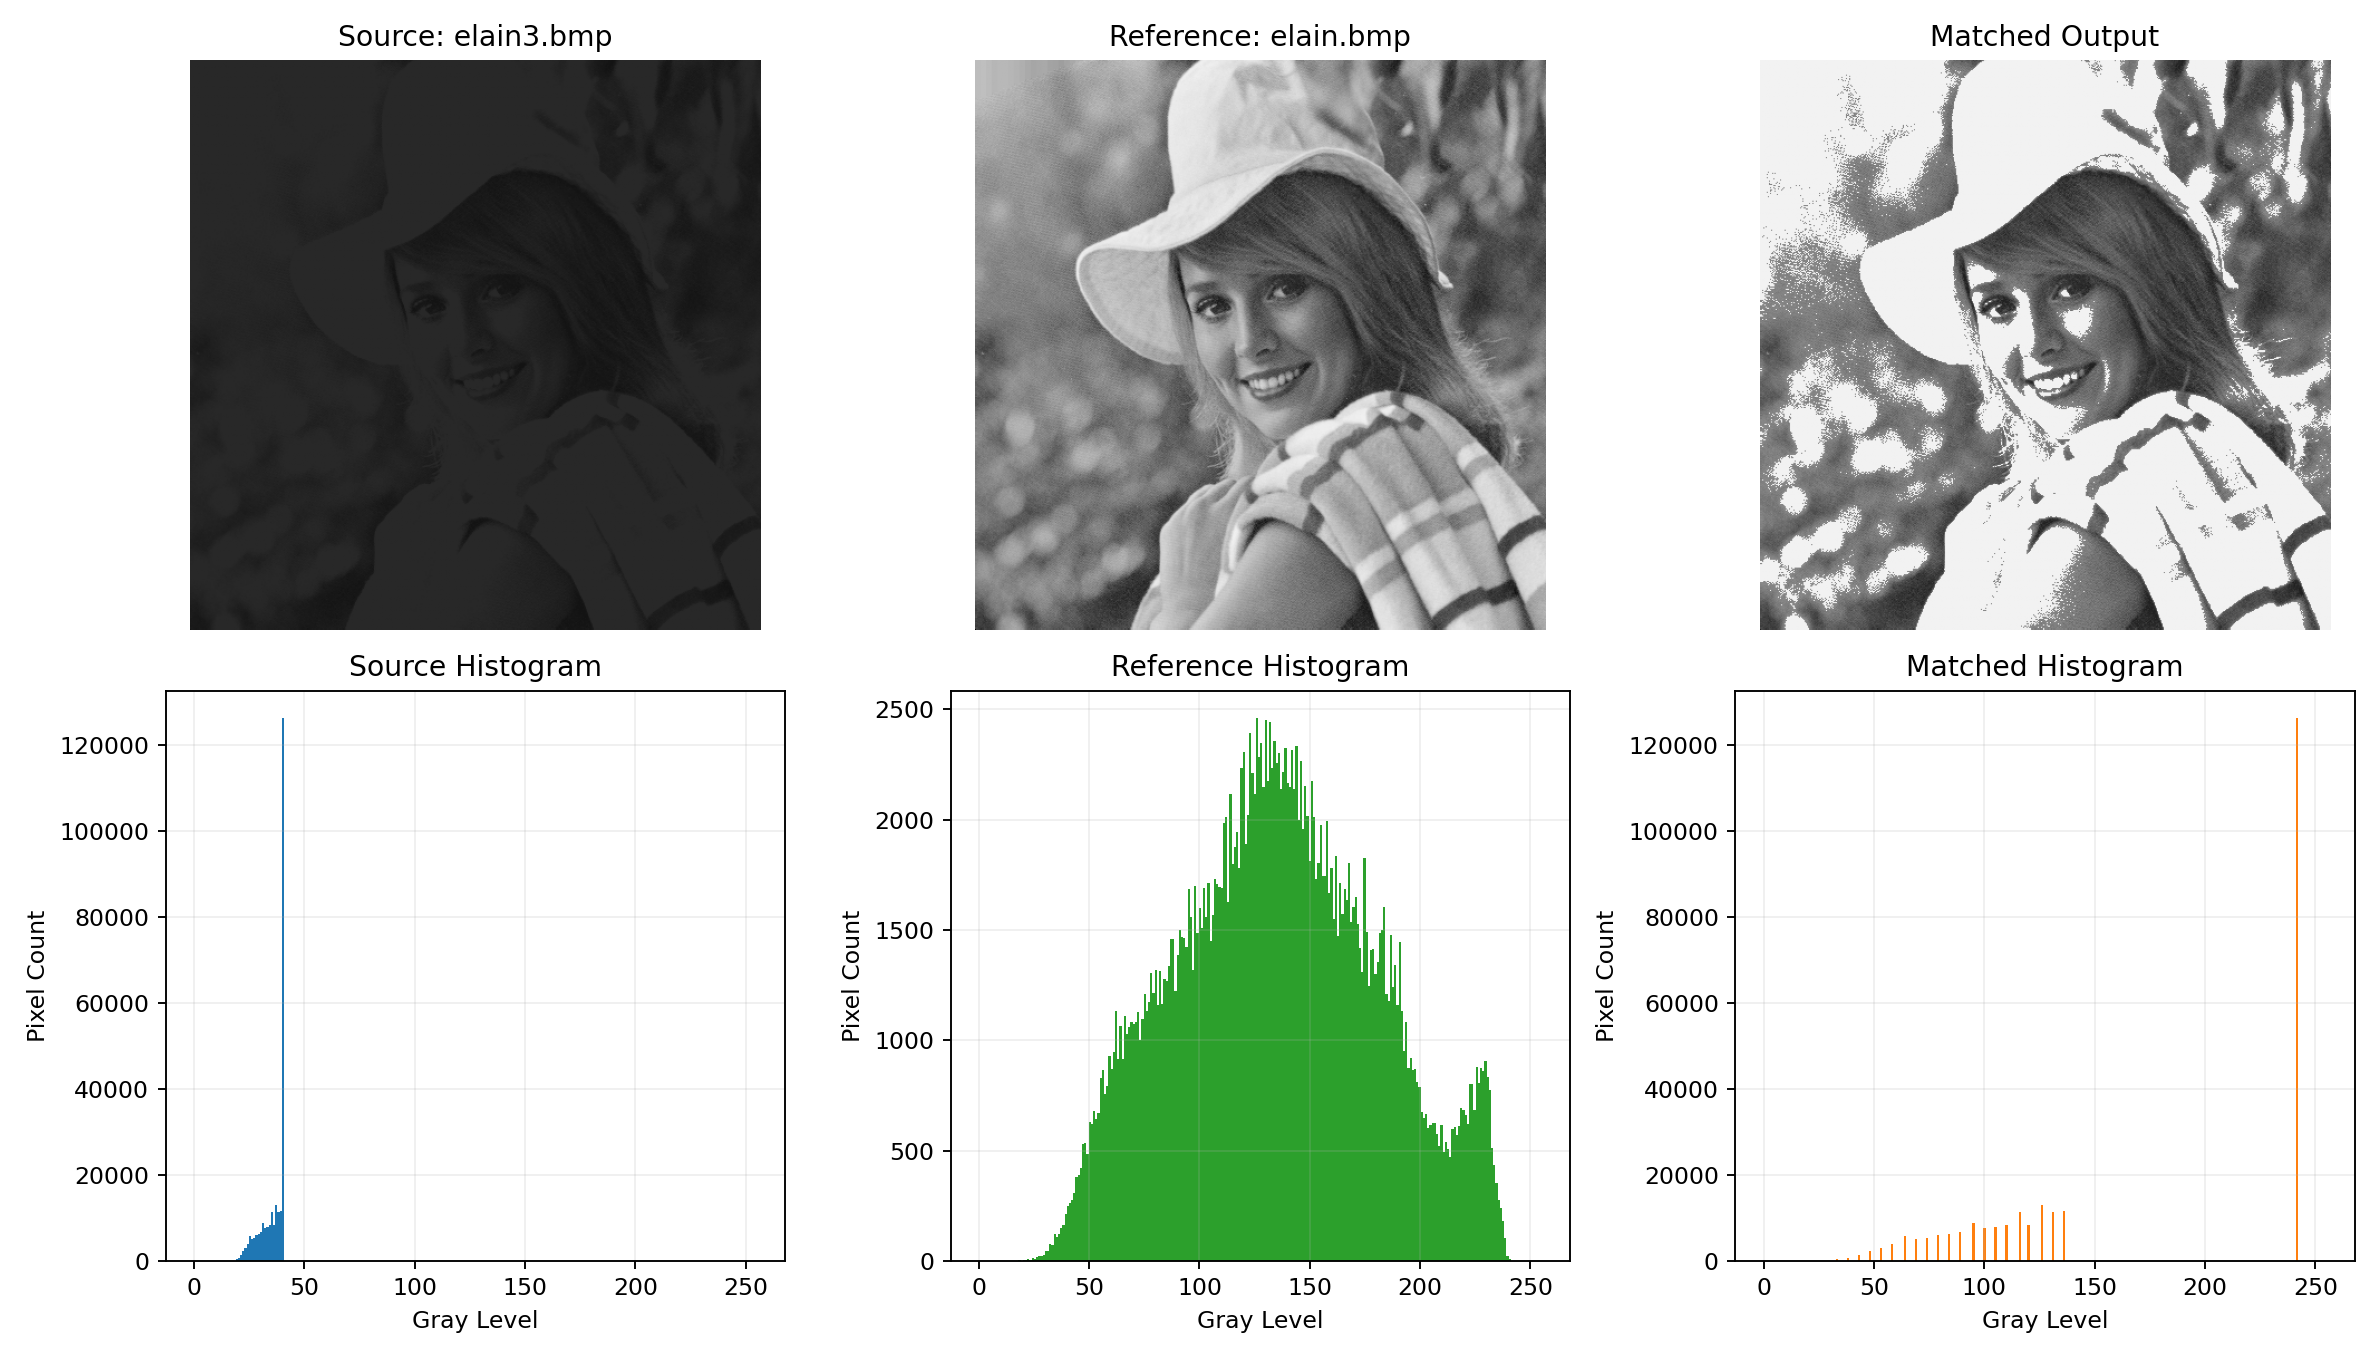
\includegraphics[width=\linewidth]{elain3_to_elain_comparison.png}
    \caption{elain3 $\rightarrow$ elain}
  \end{subfigure}
  \begin{subfigure}{0.49\textwidth}
    \centering
    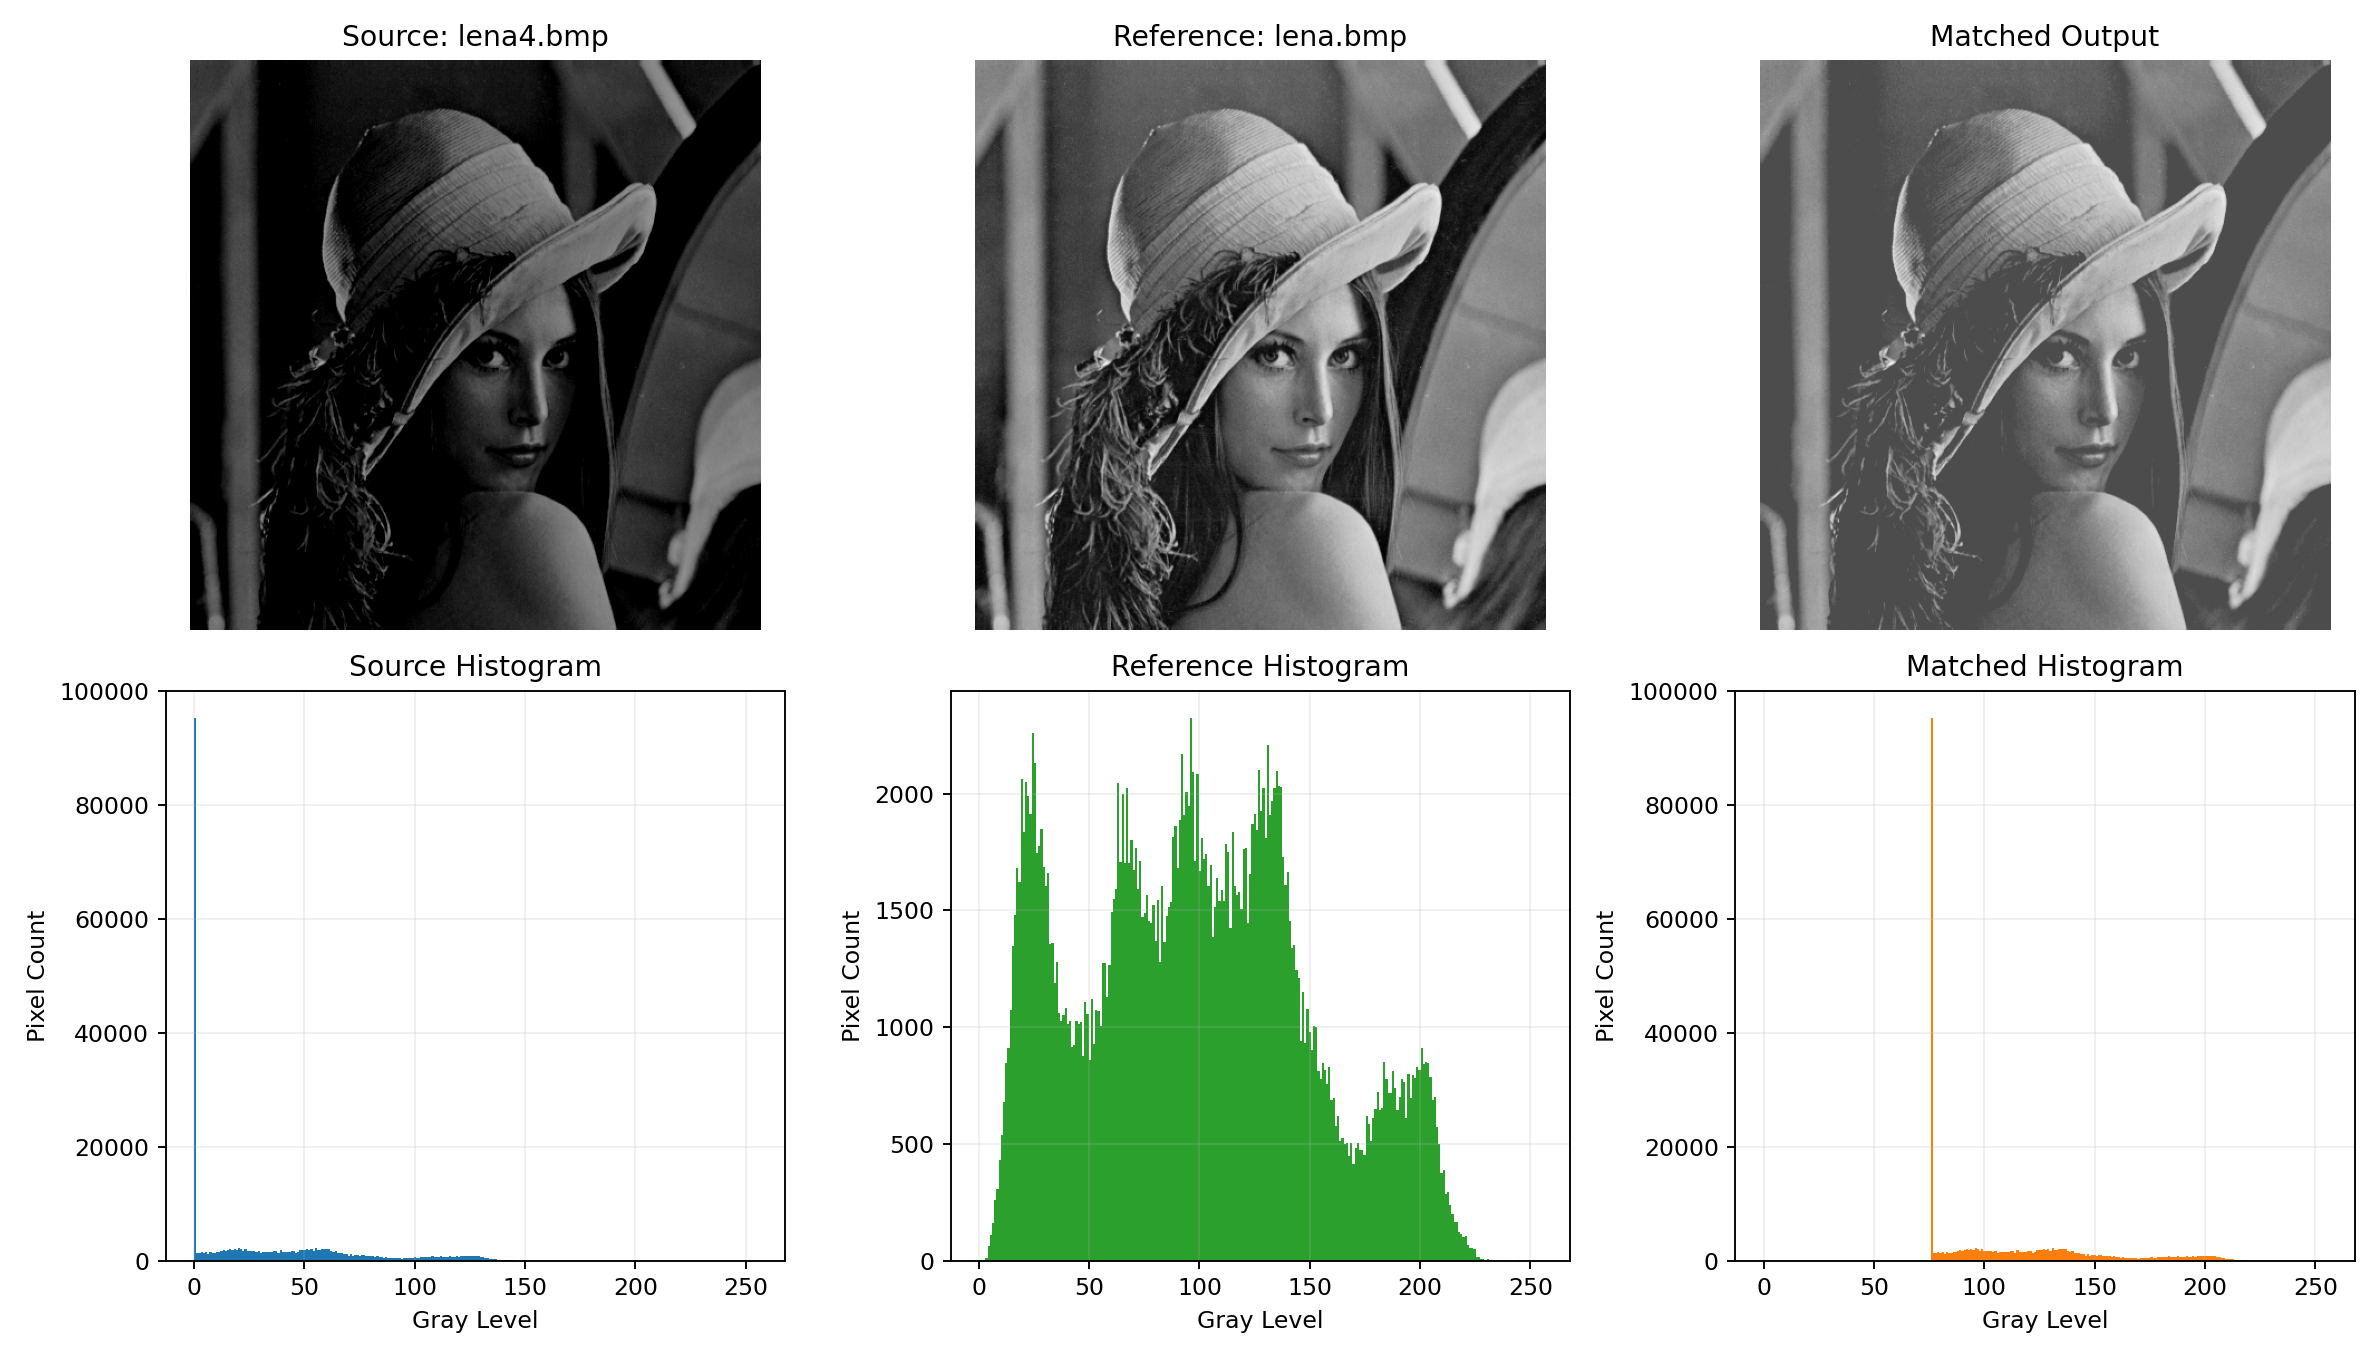
\includegraphics[width=\linewidth]{lena4_to_lena_comparison.png}
    \caption{lena4 $\rightarrow$ lena}
  \end{subfigure}

  \vspace{0.5em}
  \begin{subfigure}{0.49\textwidth}
    \centering
    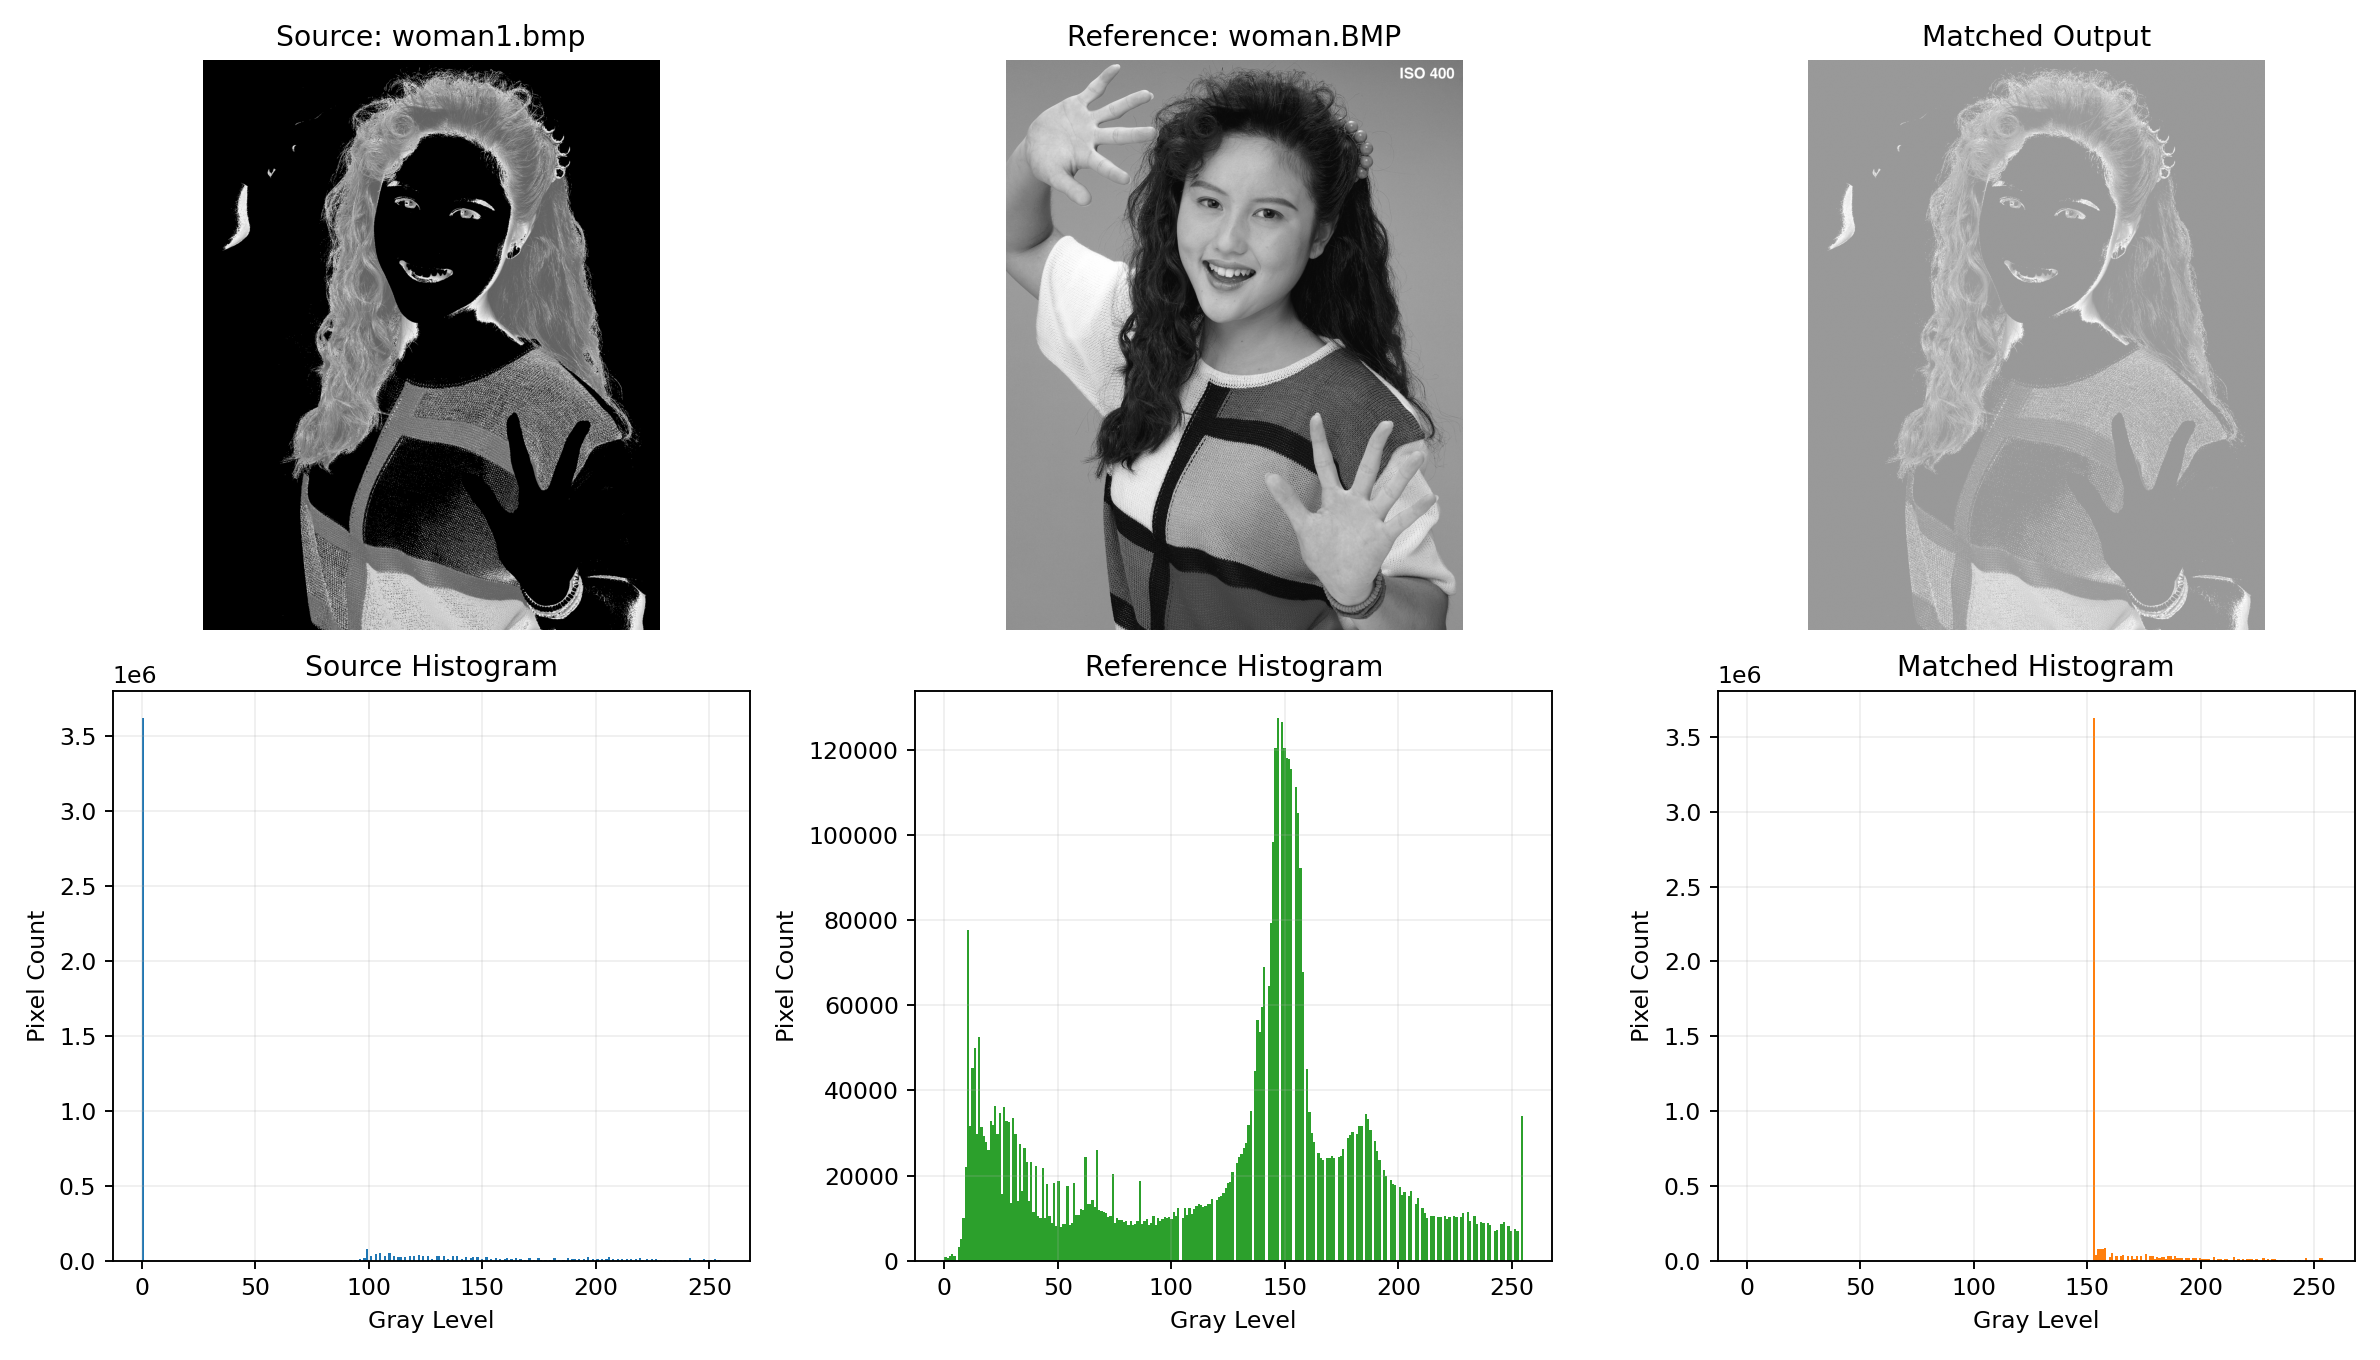
\includegraphics[width=\linewidth]{woman1_to_woman_comparison.png}
    \caption{woman1 $\rightarrow$ woman}
  \end{subfigure}
  \caption{任务3：直方图匹配结果示例}
\end{figure}

匹配后图像整体亮度和对比度更接近参考原图的统计分布，偏暗图像视觉改善较明显。

\subsection{任务4：7x7 局部直方图增强}
\begin{figure}[H]
  \centering
  \begin{subfigure}{0.49\textwidth}
    \centering
    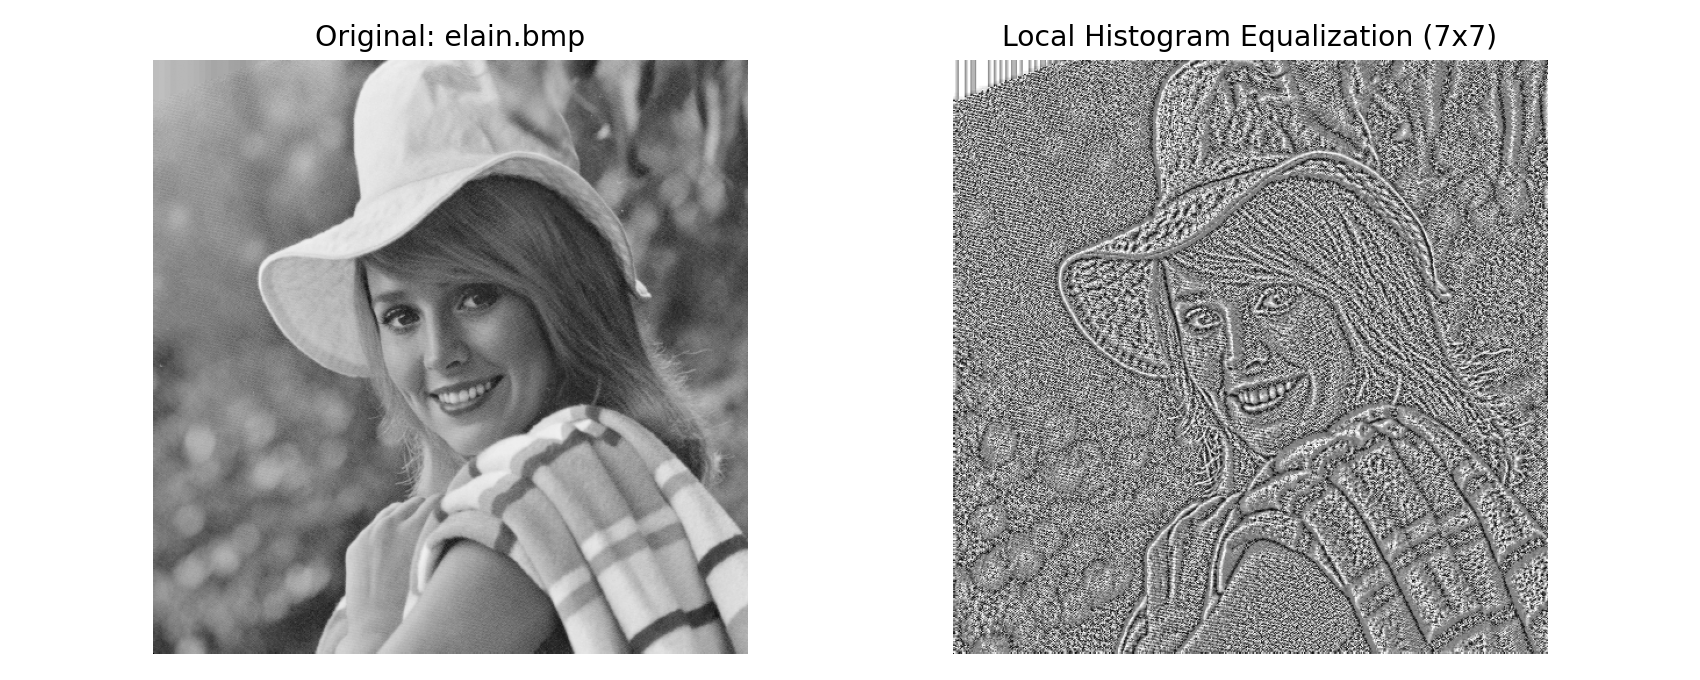
\includegraphics[width=\linewidth]{elain_local7x7_compare.png}
    \caption{elain.bmp}
  \end{subfigure}
  \begin{subfigure}{0.49\textwidth}
    \centering
    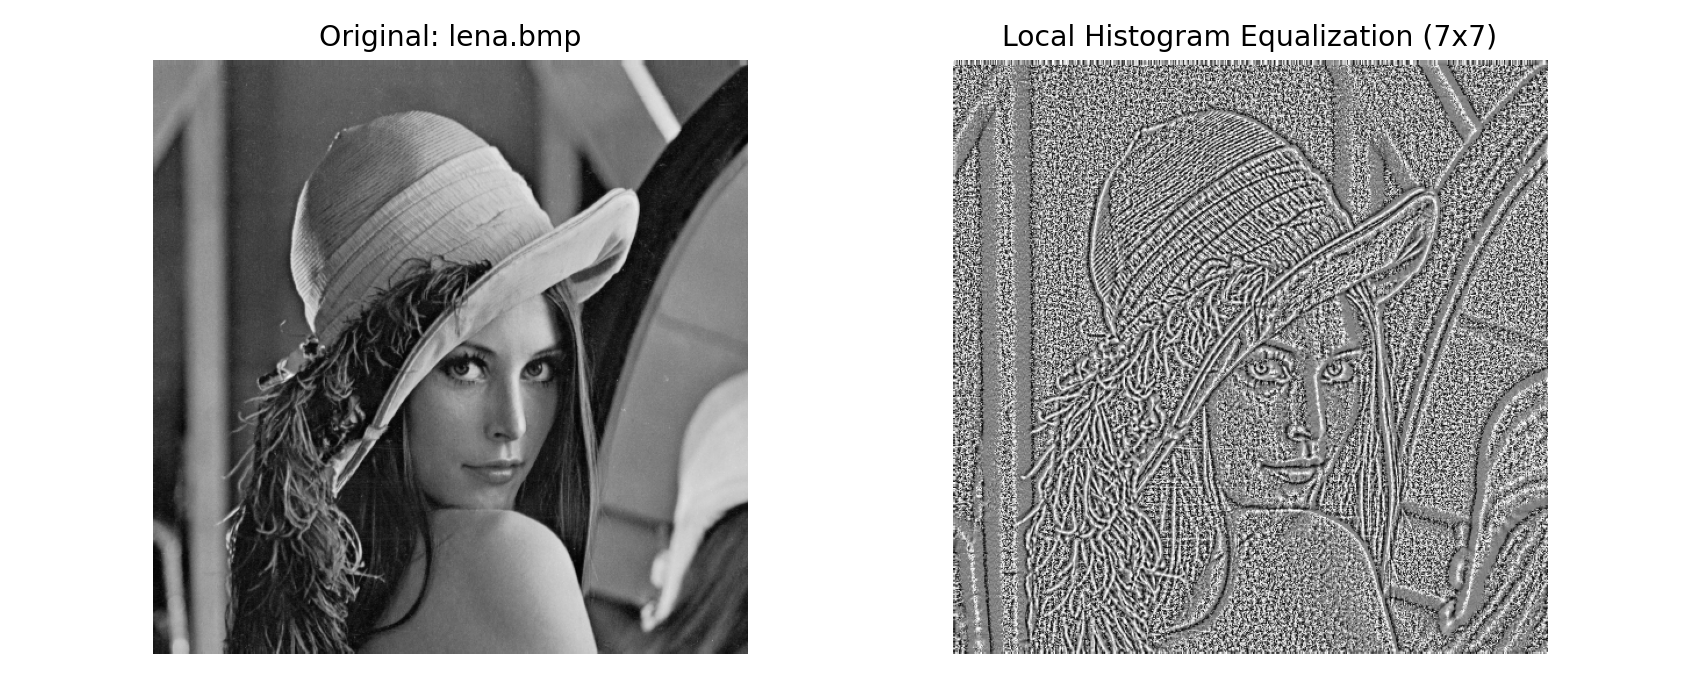
\includegraphics[width=\linewidth]{lena_local7x7_compare.png}
    \caption{lena.bmp}
  \end{subfigure}
  \caption{任务4：局部增强前后对比}
\end{figure}

\begin{table}[H]
\centering
\caption{任务4统计}
\begin{tabular}{lcc}
\toprule
图像 & 原始std & 局部增强后std \\
\midrule
elain.bmp & 46.050 & 63.200 \\
lena.bmp & 52.878 & 63.084 \\
\bottomrule
\end{tabular}
\end{table}

\subsection{任务5：基于直方图分割}
\begin{figure}[H]
  \centering
  \begin{subfigure}{0.49\textwidth}
    \centering
    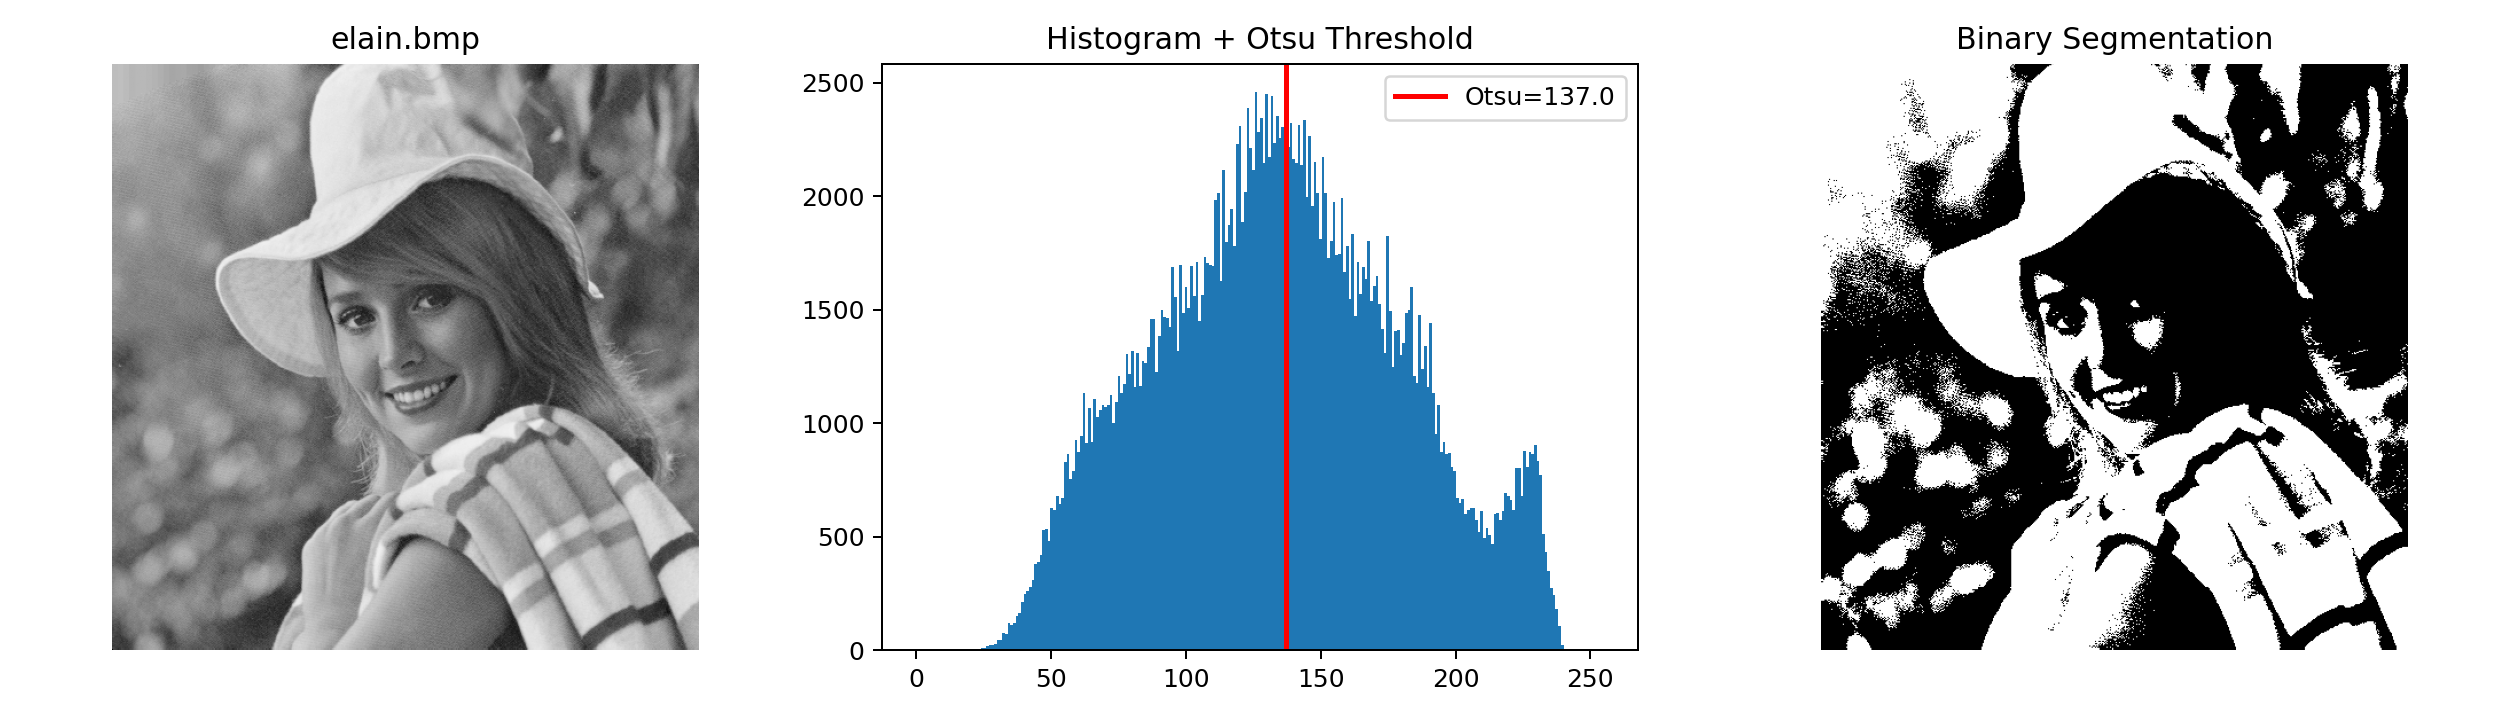
\includegraphics[width=\linewidth]{elain_segmentation_overview.png}
    \caption{elain：Otsu 二值分割}
  \end{subfigure}
  \begin{subfigure}{0.49\textwidth}
    \centering
    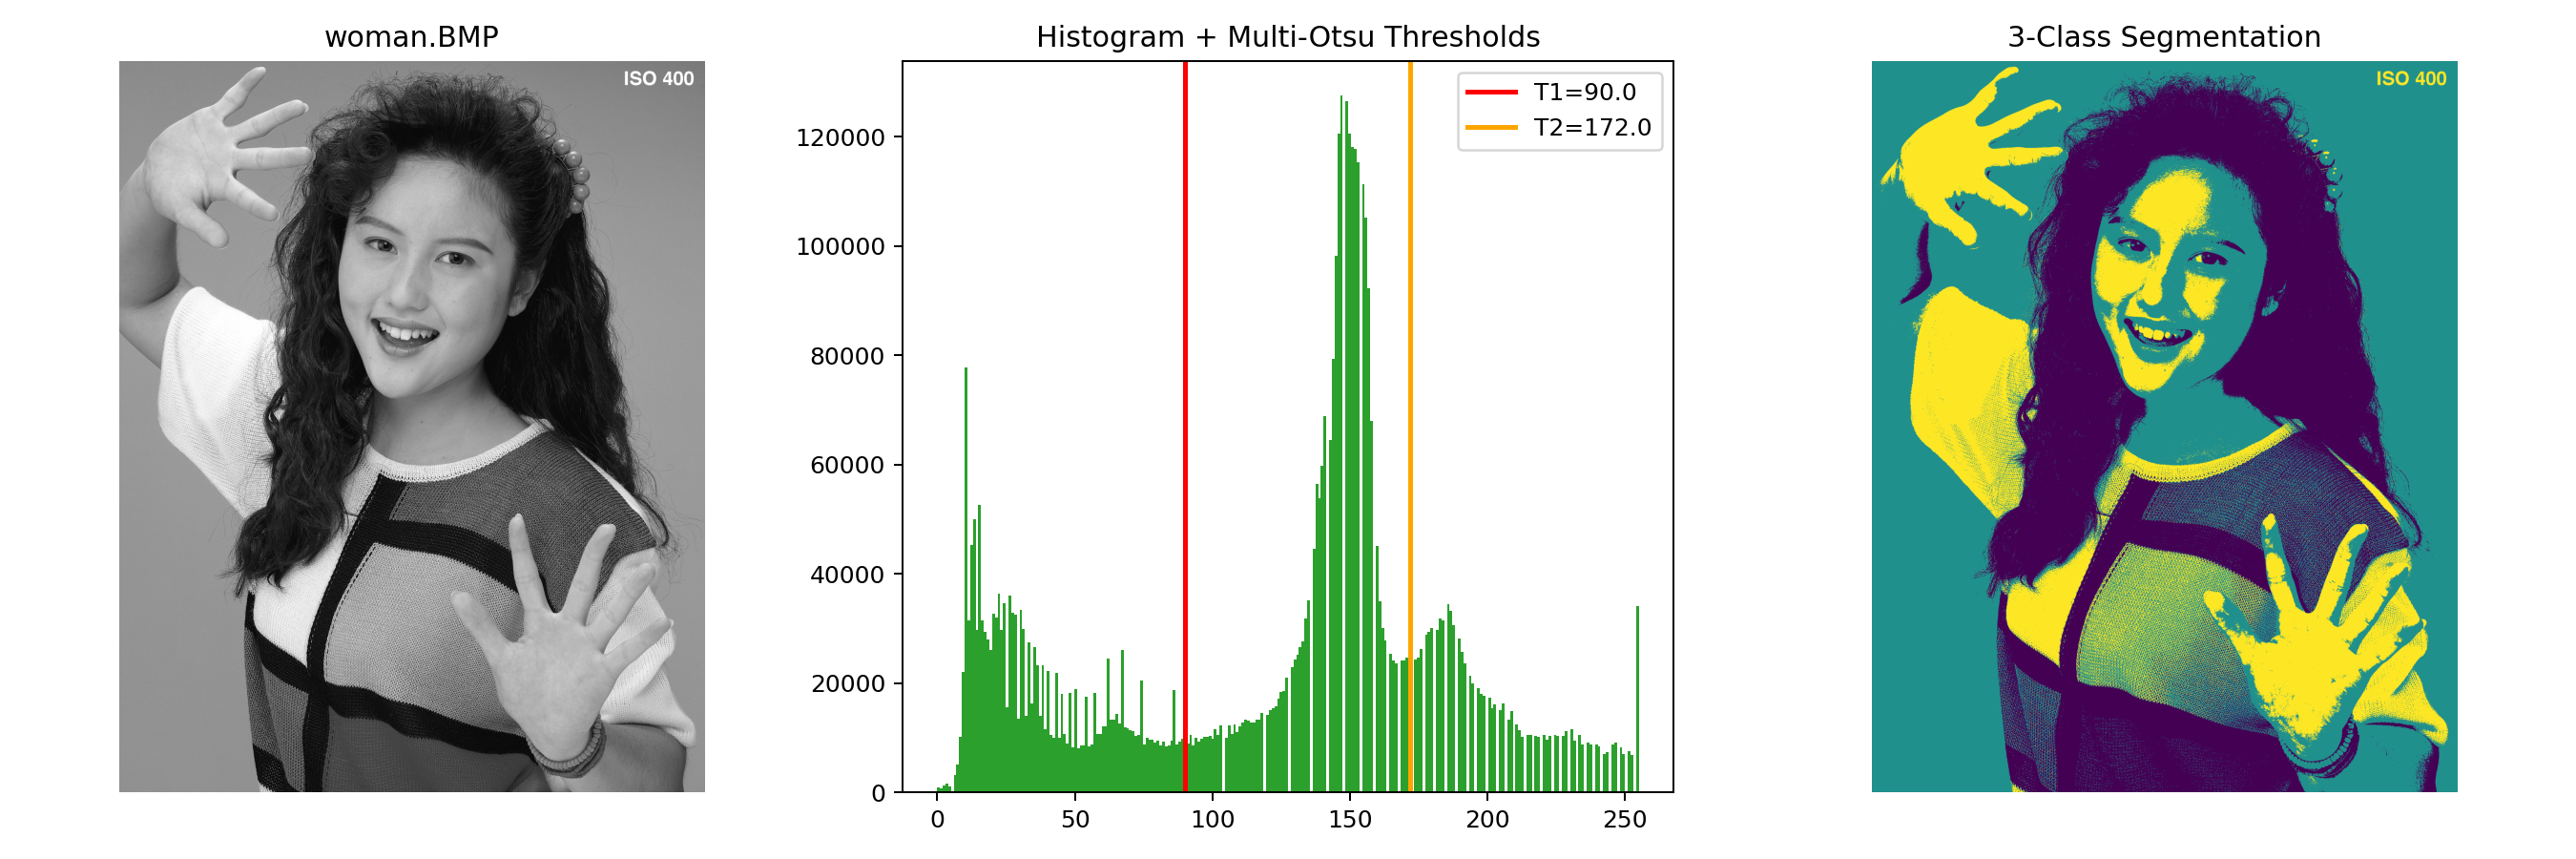
\includegraphics[width=\linewidth]{woman_segmentation_overview.png}
    \caption{woman：Multi-Otsu 三类分割}
  \end{subfigure}
  \caption{任务5分割结果}
\end{figure}

\begin{table}[H]
\centering
\caption{任务5阈值结果}
\begin{tabular}{lccc}
\toprule
图像 & 方法 & 阈值 & 前景比例 \\
\midrule
elain.bmp & Otsu & $T=137$ & 0.4824 \\
woman.BMP & Multi-Otsu(3类) & $T_1=90,\ T_2=172$ & 0.1872（高灰度类） \\
\bottomrule
\end{tabular}
\end{table}

\section{结论}
\begin{enumerate}
  \item 全局均衡对低对比度图像效果明显，但对已严重偏态分布图像可能产生过增强或亮度漂移。
  \item 直方图匹配在有参考图时更可控，能把退化图像拉向目标风格。
  \item $7\times7$ 局部增强能有效提升局部细节与纹理可见性。
  \item Otsu 与 Multi-Otsu 可快速完成基于直方图的分割任务，满足本次作业要求。
\end{enumerate}

\section*{附：编译与使用说明}
\begin{itemize}
  \item 建议在 Overleaf 选择 \textbf{XeLaTeX} 编译器。
  \item 上传本文件 \texttt{report\_hw3\_overleaf.tex}、\texttt{outputs/} 整个目录，以及原始图像文件（可选）。
  \item 若路径变化，请同步修改导言区 \texttt{\textbackslash graphicspath}。
\end{itemize}

\end{document}
